\section{VGG16}

As outlined in section \ref{sec:architectures} the pre-trained VGG16 network will serve as the base-line comparison for this work. We chose VGG16 as it has a tried and true performance on labeled AT-TPC data from the $^{46}Ar$ experiment.(\cite{Kuchera2019}). For each labeled dataset listed in section \ref{sec:data} a logistic regression model was fit to the respective VGG16-representation. To estimate the variability in the result a K-fold cross validation approach was taken, with $K=5$. We report test-$f1$ scores for each class and average for the classification. The results are listed in table \ref{tab:vgg_results}

\begin{table}
\centering
\begin{tabular}{lllll}
\toprule
{} & Proton & Carbon & Other & All \\
\midrule
Simulated &  $\underset{\num{+- 1.014e-03 }  }{\num{ 0.999 } }$ &  $\underset{\num{+- 1.029e-03 }  }{\num{ 0.999 } }$ &  N/A &  $\underset{\num{+- 1.022e-03 }  }{\num{ 0.999 } }$ \\
Filtered  &  $\underset{\num{+- 5.108e-02 }  }{\num{ 0.918 } }$ &  $\underset{\num{+- 4.267e-02 }  }{\num{ 0.69 } }$ &  $\underset{\num{+- 2.359e-02 }  }{\num{ 0.908 } }$ &  $\underset{\num{+- 3.911e-02 }  }{\num{ 0.839 } }$ \\
Full      &  $\underset{\num{+- 4.653e-02 }  }{\num{ 0.84 } }$ &  $\underset{\num{+- 4.860e-02 }  }{\num{ 0.668 } }$ &  $\underset{\num{+- 1.730e-02 }  }{\num{ 0.89 } }$ &  $\underset{\num{+- 3.748e-02 }  }{\num{ 0.799 } }$ \\
\bottomrule
\end{tabular}
\caption[VGG classification results]{Logistic regression classification results using the VGG16 representation of the labeled data listed in section \ref{sec:data}. The error is given as the standard deviation in the $f1$ score over the $K=5$ folds of cross validation.}\label{tab:vgg_results}
\end{table}

 Additionally the scarceness of labeled data begs the question of how much labeled data is needed to achieve strong classification. To estimate this relationship we sample increasing subsets of the labeled data, each containing the previously selected data. For each selection a logistic regression model is fit and a $f1$ core is computed. This procedure is sensitive to which subset selected for fitting first and so a variability estimate is computed by running this procedure $N=100$ times. We report the mean and standard deviation for each dataset. The result of this analysis is shown in figure \ref{fig:vgg_n_samples}


\begin{figure}
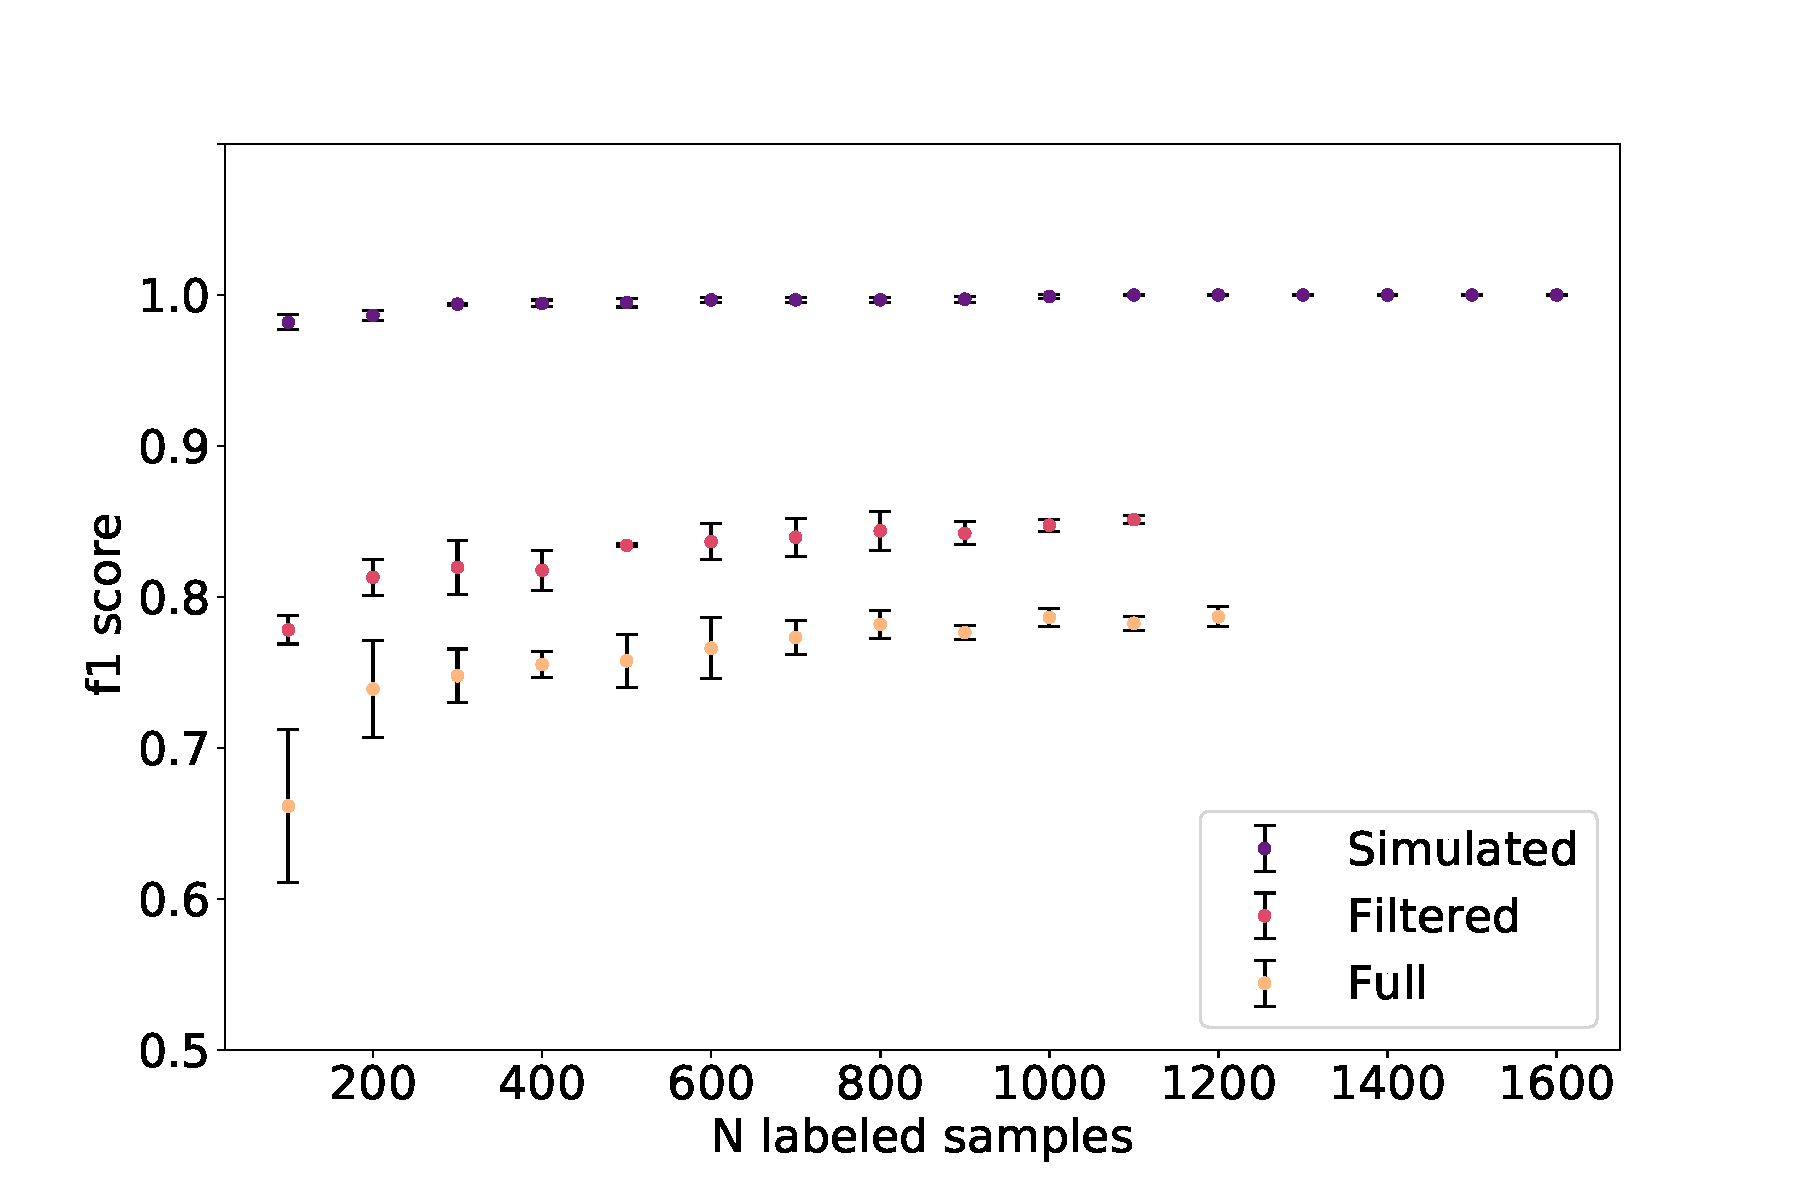
\includegraphics[width=\textwidth]{plots/vgg_n_samples.pdf}
\caption[VGG16 performance on labeled subsets]{VGG16 performance on increasing subsets of labeled data. The error-bars represent the $\pm 1\sigma$ interval. The y axis $f1$ score is computed as the unweighted average of the sample classes.}\label{fig:vgg_n_samples}
\end{figure}